\documentclass[11pt,a4paper]{report}
\usepackage[textwidth=37em,vmargin=30mm]{geometry}
\usepackage{calc,xunicode,amsmath,amssymb,paralist,enumitem,tabu,booktabs,datetime2,xeCJK,xeCJKfntef,listings}
\usepackage{tocloft,fancyhdr,tcolorbox,xcolor,graphicx,eso-pic,xltxtra,xelatexemoji}

\newcommand{\envyear}[0]{2024}
\newcommand{\envdatestr}[0]{2024-10-28}
\newcommand{\envfinaldir}[0]{webdb/2024/20241028/final}

\usepackage[hidelinks]{hyperref}
\hypersetup{
    colorlinks=false,
    pdfpagemode=FullScreen,
    pdftitle={Web Digest - \envdatestr}
}

\setlength{\cftbeforechapskip}{10pt}
\renewcommand{\cftchapfont}{\rmfamily\bfseries\large\raggedright}
\setlength{\cftbeforesecskip}{2pt}
\renewcommand{\cftsecfont}{\sffamily\small\raggedright}

\setdefaultleftmargin{2em}{2em}{1em}{1em}{1em}{1em}

\usepackage{xeCJK,xeCJKfntef}
\xeCJKsetup{PunctStyle=plain,RubberPunctSkip=false,CJKglue=\strut\hskip 0pt plus 0.1em minus 0.05em,CJKecglue=\strut\hskip 0.22em plus 0.2em}
\XeTeXlinebreaklocale "zh"
\XeTeXlinebreakskip = 0pt


\setmainfont{Brygada 1918}
\setromanfont{Brygada 1918}
\setsansfont{IBM Plex Sans}
\setmonofont{JetBrains Mono NL}
\setCJKmainfont{Noto Serif CJK SC}
\setCJKromanfont{Noto Serif CJK SC}
\setCJKsansfont{Noto Sans CJK SC}
\setCJKmonofont{Noto Sans CJK SC}

\setlength{\parindent}{0pt}
\setlength{\parskip}{8pt}
\linespread{1.15}

\lstset{
	basicstyle=\ttfamily\footnotesize,
	numbersep=5pt,
	backgroundcolor=\color{black!5},
	showspaces=false,
	showstringspaces=false,
	showtabs=false,
	tabsize=2,
	captionpos=b,
	breaklines=true,
	breakatwhitespace=true,
	breakautoindent=true,
	linewidth=\textwidth
}






\newcommand{\coverpic}[2]{
    % argv: itemurl, authorname
    Cover photo by #2~~(\href{#1}{#1})
}
\newcommand{\makeheader}[0]{
    \begin{titlepage}
        % \newgeometry{hmargin=15mm,tmargin=21mm,bmargin=12mm}
        \begin{center}
            
            \rmfamily\scshape
            \fontspec{BaskervilleF}
            \fontspec{Old Standard}
            \fontsize{59pt}{70pt}\selectfont
            WEB\hfill DIGEST
            
            \vfill
            % \vskip 30pt
            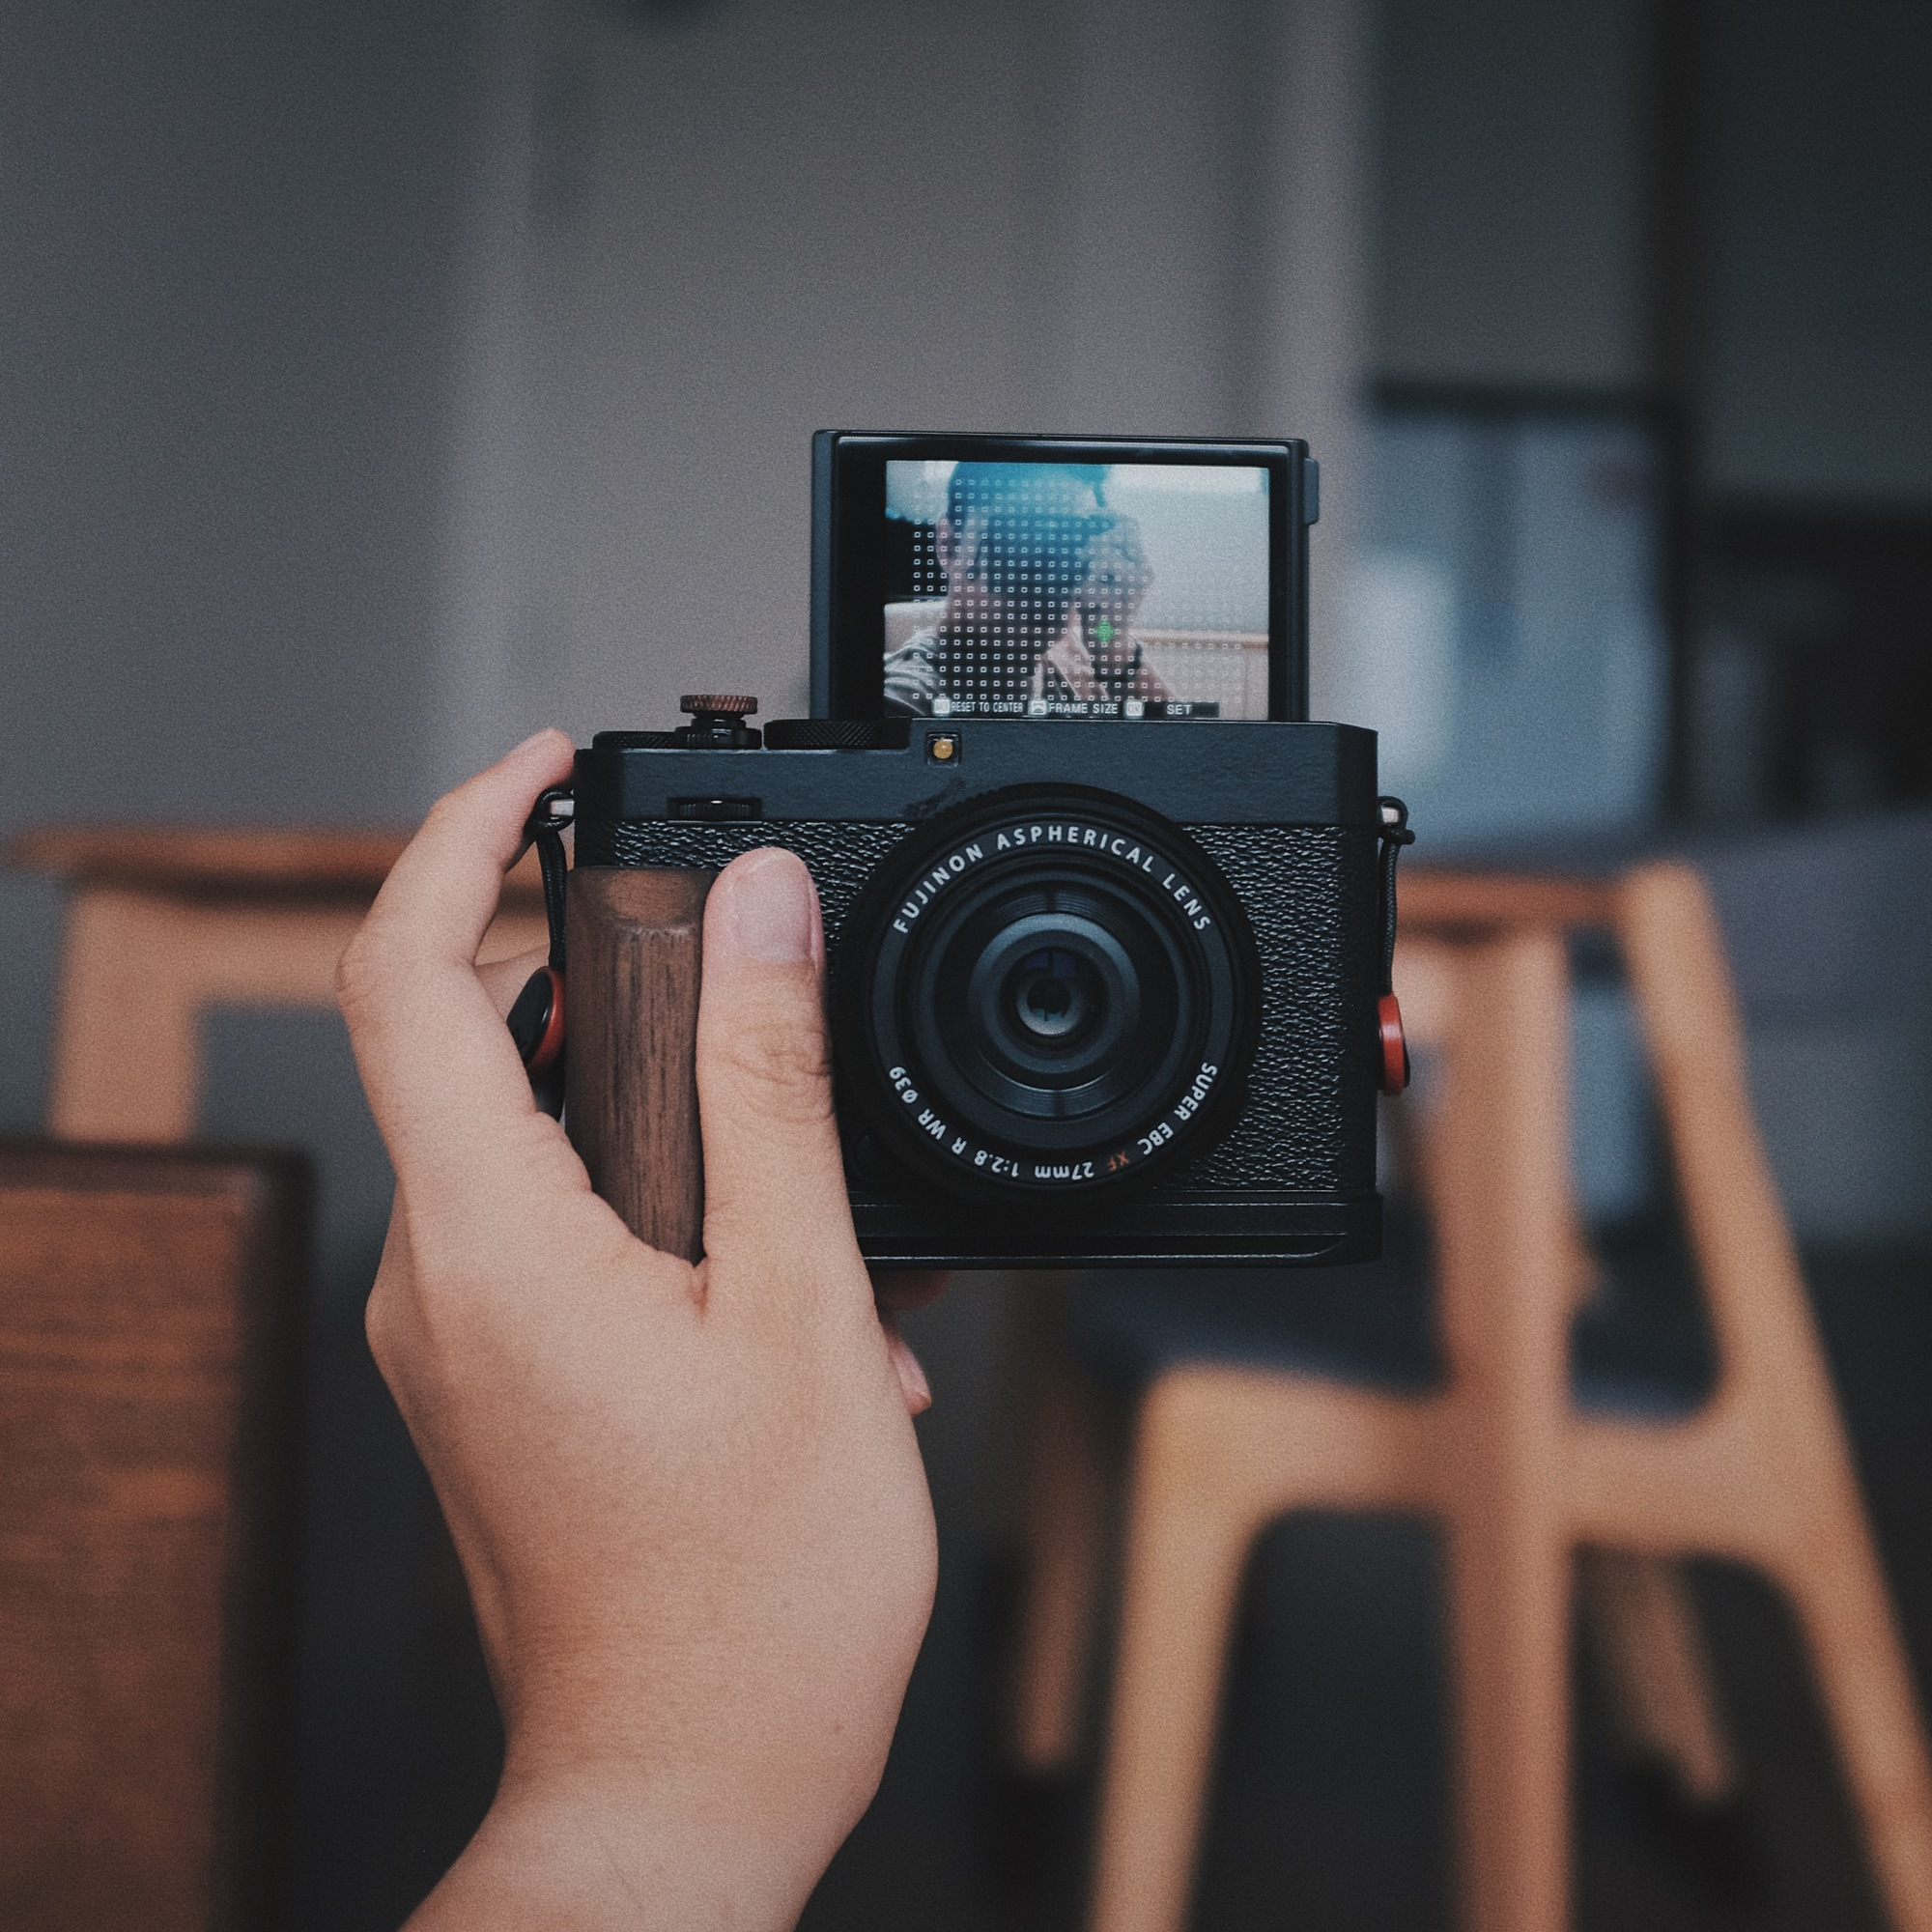
\includegraphics[width=\linewidth]{\envfinaldir/coverpic-prod.jpg}\par
            % \vskip 30pt
            \vfill

            \normalsize\rmfamily\scshape
            \copyright{} The Web Digest Project \hfill\large \envdatestr
        \end{center}
    \end{titlepage}
    % \restoregeometry
}
\newcommand{\simplehref}[1]{%
    \textcolor{blue!80!green}{\href{#1}{#1}}%
}
\renewcommand{\contentsname}{\center\Huge\sffamily\bfseries Contents\par\vskip 20pt}
\newcounter{ipartcounter}
\setcounter{ipartcounter}{0}
\newcommand{\ipart}[1]{
    % \vskip 20pt
    \clearpage
    \stepcounter{ipartcounter}
    \phantomsection
    \addcontentsline{toc}{chapter}{#1}
    % \begin{center}
    %     \Huge
    %     \sffamily\bfseries
    %     #1
    % \end{center}
    % \vskip 20pt plus 7pt
}
\newcounter{ichaptercounter}
\setcounter{ichaptercounter}{0}
\newcommand{\ichapter}[1]{
    % \vskip 20pt
    \clearpage
    \stepcounter{ichaptercounter}
    \phantomsection
    \addcontentsline{toc}{section}{\numberline{\arabic{ichaptercounter}}#1}
    \begin{center}
        \Huge
        \sffamily\bfseries
        #1
    \end{center}
    \vskip 20pt plus 7pt
}
\newcommand{\entrytitlefont}[1]{\subsection*{\raggedright\Large\sffamily\bfseries#1}}
\newcommand{\entryitemGeneric}[2]{
    % argv: title, url
    \parbox{\linewidth}{
        \entrytitlefont{#1}\par\vskip 5pt
        \footnotesize\ttfamily\mdseries
        \simplehref{#2}
    }\vskip 11pt plus 11pt minus 1pt
}
\newcommand{\entryitemGithub}[3]{
    % argv: title, url, desc
    \parbox{\linewidth}{
        \entrytitlefont{#1}\par\vskip 5pt
        \footnotesize\ttfamily\mdseries
        \simplehref{#2}\par\vskip 5pt
        \small\rmfamily\mdseries#3
    }\vskip 11pt plus 11pt minus 1pt
}
\newcommand{\entryitemAp}[3]{
    % argv: title, url, desc
    \parbox{\linewidth}{
        \entrytitlefont{#1}\par\vskip 5pt
        \footnotesize\ttfamily\mdseries
        \simplehref{#2}\par\vskip 5pt
        \small\rmfamily\mdseries#3
    }\vskip 11pt plus 11pt minus 1pt
}
\newcommand{\entryitemHackernews}[3]{
    % argv: title, hnurl, rawurl
    % \parbox{\linewidth}{
    %     \entrytitlefont{#1}\par\vskip 5pt
    %     \footnotesize\ttfamily\mdseries
    %     \simplehref{#3}\par
    %     \textcolor{black!50}{\href{#2}{#2}}
    % }\vskip 11pt plus 11pt minus 1pt
    \begin{minipage}{\linewidth}
            \entrytitlefont{#1}\par\vskip 5pt
            \footnotesize\ttfamily\mdseries
            \simplehref{#3}\par
            \textcolor{black!50}{\href{#2}{#2}}
    \end{minipage}\par\vskip 11pt plus 11pt minus 1pt
}







\begin{document}

\makeheader

\tableofcontents\clearpage




\ipart{Developers}
\ichapter{Hacker News}
\entryitemTwoLinks{Up to \$41B in World Bank climate finance unaccounted for, Oxfam finds}{https://news.ycombinator.com/item?id=41964639}{https://www.oxfam.org/en/press-releases/41-billion-world-bank-climate-finance-unaccounted-oxfam-finds}

\entryitemTwoLinks{Ibis: Federated Wikipedia alternative}{https://news.ycombinator.com/item?id=41964210}{https://ibis.wiki/article/Announcing\_Ibis,\_the\_federated\_Wikipedia\_Alternative}

\entryitemTwoLinks{Freenet: A decentralized alternative to world wide web}{https://news.ycombinator.com/item?id=41964191}{https://freenet.org/}

\entryitemTwoLinks{Using SQLite as storage for web server static content}{https://news.ycombinator.com/item?id=41963996}{https://clace.io/blog/sqlite/}

\entryitemTwoLinks{NewPipe on Linux, Using Android\_translation\_layer}{https://news.ycombinator.com/item?id=41963932}{https://flathub.org/apps/net.newpipe.NewPipe}

\entryitemTwoLinks{School is Not Enough: Learning is a consequence of doing (2021)}{https://news.ycombinator.com/item?id=41963063}{https://map.simonsarris.com/p/school-is-not-enough}

\entryitemTwoLinks{50 Years Ago, Sugar Industry Paid Scientists to Point Blame at Fat (2016)}{https://news.ycombinator.com/item?id=41962750}{https://www.npr.org/sections/thetwo-way/2016/09/13/493739074/50-years-ago-sugar-industry-quietly-paid-scientists-to-point-blame-at-fat}

\entryitemTwoLinks{You-get: Dumb downloader that scrapes the web}{https://news.ycombinator.com/item?id=41962205}{https://github.com/soimort/you-get}

\entryitemTwoLinks{A Chopin waltz unearthed after nearly 200 years}{https://news.ycombinator.com/item?id=41961866}{https://www.nytimes.com/2024/10/27/arts/music/chopin-waltz-discovery.html}

\entryitemTwoLinks{Crossing the USA by Train}{https://news.ycombinator.com/item?id=41961034}{https://blinry.org/coast-to-coast/}

\entryitemTwoLinks{Writes and Write-Nots}{https://news.ycombinator.com/item?id=41960914}{https://paulgraham.com/writes.html}

\entryitemTwoLinks{Open Source on its own is no alternative to Big Tech}{https://news.ycombinator.com/item?id=41960442}{https://berthub.eu/articles/posts/open-source-by-itself-is-no-alternative-for-big-tech/}

\entryitemTwoLinks{Moonshine, the new state of the art for speech to text}{https://news.ycombinator.com/item?id=41960085}{https://petewarden.com/2024/10/21/introducing-moonshine-the-new-state-of-the-art-for-speech-to-text/}

\entryitemTwoLinks{Typeset: An HTML pre-proces­sor for web ty­pog­ra­phy}{https://news.ycombinator.com/item?id=41960010}{https://typeset.lllllllllllllllll.com/}

\entryitemTwoLinks{We shrunk our Javascript monorepo git size}{https://news.ycombinator.com/item?id=41959428}{https://www.jonathancreamer.com/how-we-shrunk-our-git-repo-size-by-94-percent/}

\entryitemTwoLinks{Character amnesia in China}{https://news.ycombinator.com/item?id=41959256}{https://globalchinapulse.net/character-amnesia-in-china/}

\entryitemTwoLinks{I discovered mysterious hidden signals on a public radio channel (2013) [video]}{https://news.ycombinator.com/item?id=41958766}{https://media.ccc.de/v/30C3\_-\_5588\_-\_en\_-\_saal\_g\_-\_201312281600\_-\_my\_journey\_into\_fm-rds\_-\_oona\_raisanen}

\entryitemTwoLinks{James Webb Telescope discovers some quasars that seem to exist in isolation}{https://news.ycombinator.com/item?id=41958593}{https://scitechdaily.com/james-webb-telescope-discovers-quasars-where-they-shouldnt-exist/}

\entryitemTwoLinks{ZombAIs: From Prompt Injection to C2 with Claude Computer Use}{https://news.ycombinator.com/item?id=41958550}{https://embracethered.com/blog/posts/2024/claude-computer-use-c2-the-zombais-are-coming/}

\entryitemTwoLinks{ADHD and managing your professional reputation}{https://news.ycombinator.com/item?id=41958221}{https://www.optimaloutliers.com/p/adhd-and-managing-your-reputation}\ichapter{Phoronix}
\entryitemGeneric{\hskip 0pt{}Linux 6.12-rc5 Released With Intel LAM Disabled, ASUS Lunar Lake Laptop Performance Fix}{https://www.phoronix.com/news/Linux-6.12-rc5-Released}

\entryitemGeneric{\hskip 0pt{}Linux Working On A Counter To Keep Track Of The Number Of Hung Tasks Since Boot}{https://www.phoronix.com/news/Linux-hung\_task\_detect\_count}

\entryitemGeneric{\hskip 0pt{}Linux 6.12-rc5 Disabling Intel's Linear Address Masking "LAM" Due To Security Concerns}{https://www.phoronix.com/news/Linux-Disabling-Intel-LAM}

\entryitemGeneric{\hskip 0pt{}Intel's PCIe Cooling Driver Ready For Linux 6.13 To Reduce Bandwidth When Running Hot}{https://www.phoronix.com/news/Linux-6.13-PCIe-Cooling-Driver}

\entryitemGeneric{\hskip 0pt{}Linux NETFS Patches Help With CIFS Performance, Single Blob Objects}{https://www.phoronix.com/news/Linux-NETFS-Better-Reads}

\entryitemGeneric{\hskip 0pt{}DM-INLINECRYPT Being Worked On To Leverage Inline Block Device Encryption}{https://www.phoronix.com/news/DM-INLINECRYPT-Patches}

\entryitemGeneric{\hskip 0pt{}Vulkan 1.3.300 Delivers New Cooperative Matrix Extension From NVIDIA}{https://www.phoronix.com/news/Vulkan-1.3.300-Released}

\entryitemGeneric{\hskip 0pt{}Initial Intel Xe3 OpenGL \& Vulkan Driver Code Submitted For Mesa 24.3}{https://www.phoronix.com/news/Mesa-24.3-Initial-Intel-Xe3-PTL}

\entryitemGeneric{\hskip 0pt{}ASUS WMI Fix Submitted For Linux 6.12-rc5 To Handle Lunar Lake Performance Issue}{https://www.phoronix.com/news/Linux-6.12-rc5-ASUS-Platform}


\ipart{Developers~~~~(zh-Hans)}
\ichapter{Solidot}
\entryitemGeneric{\hskip 0pt{}NASA 研发能从轨道降落的火星直升机}{https://www.solidot.org/story?sid=79601}

\entryitemGeneric{\hskip 0pt{}OnlyFans 支付给歌手的钱超过了 Spotify}{https://www.solidot.org/story?sid=79600}

\entryitemGeneric{\hskip 0pt{}天文学家在星际空间发现复杂碳分子}{https://www.solidot.org/story?sid=79599}

\entryitemGeneric{\hskip 0pt{}达美航空正式对 CrowdStrike 提起诉讼}{https://www.solidot.org/story?sid=79598}

\entryitemGeneric{\hskip 0pt{}波音探索出售其太空业务}{https://www.solidot.org/story?sid=79597}

\entryitemGeneric{\hskip 0pt{}Google DeepMind 构建 AI 帮助逆转政治极化}{https://www.solidot.org/story?sid=79596}

\entryitemGeneric{\hskip 0pt{}超新星可能清理过太阳系}{https://www.solidot.org/story?sid=79595}

\entryitemGeneric{\hskip 0pt{}人口峰值可能会更快到来}{https://www.solidot.org/story?sid=79594}

\entryitemGeneric{\hskip 0pt{}蒂姆波顿称互联网让他倍感抑郁}{https://www.solidot.org/story?sid=79593}

\entryitemGeneric{\hskip 0pt{}Kroger 和沃尔玛否认会使用数字价格标签动态定价}{https://www.solidot.org/story?sid=79592}

\entryitemGeneric{\hskip 0pt{}Linux 项目根据 OFAC 制裁名单移除俄罗斯维护者}{https://www.solidot.org/story?sid=79591}

\entryitemGeneric{\hskip 0pt{}报告称中国 5 个行业产能超过全球需求}{https://www.solidot.org/story?sid=79590}

\entryitemGeneric{\hskip 0pt{}碳排放增长速度超过了疫情前}{https://www.solidot.org/story?sid=79589}

\entryitemGeneric{\hskip 0pt{}2024 年 Salem 奖授予了 Miguel Walsh 和王艺霖}{https://www.solidot.org/story?sid=79588}

\entryitemGeneric{\hskip 0pt{}波音制造的一颗卫星在太空爆炸}{https://www.solidot.org/story?sid=79587}

\entryitemGeneric{\hskip 0pt{}Verisign 和 ICANN 更新了 DNS Root Zone 维护者服务协议}{https://www.solidot.org/story?sid=79586}

\entryitemGeneric{\hskip 0pt{}Google 开源其 AI 水印系统 SynthID}{https://www.solidot.org/story?sid=79585}\ichapter{V2EX}
\entryitemGeneric{\hskip 0pt{}[Apple] iMessage 聊天记录大段缺失或者说不显示}{https://www.v2ex.com/t/1084097}

\entryitemGeneric{\hskip 0pt{}[OpenAI] 聊天机器人,如何训练?}{https://www.v2ex.com/t/1084096}

\entryitemGeneric{\hskip 0pt{}[问与答] 大家有找过帽子叔叔的经历吗,关于受案回执疑问}{https://www.v2ex.com/t/1084095}

\entryitemGeneric{\hskip 0pt{}[科技] ARC 浏览器将停止开发,又要发布一款新的浏览器}{https://www.v2ex.com/t/1084094}

\entryitemGeneric{\hskip 0pt{}[酷工作] [远程] 室内家居装饰设计创业项目招前端和后端}{https://www.v2ex.com/t/1084093}

\entryitemGeneric{\hskip 0pt{}[问与答] 最优成本实现 win/mac 原生 UI 风格的库/语言是什么?}{https://www.v2ex.com/t/1084092}

\entryitemGeneric{\hskip 0pt{}[分享创造] 将苹果备忘录生成博客网站(一个想法)}{https://www.v2ex.com/t/1084091}

\entryitemGeneric{\hskip 0pt{}[问与答] WindowsHDR 显示器浏览器播放 SDR 时有几率被错误识别为 HDR}{https://www.v2ex.com/t/1084090}

\entryitemGeneric{\hskip 0pt{}[问与答] 无账户密码的内网应用(网页),使用什么技术方案可以增加用户名密码以在外网安全访问}{https://www.v2ex.com/t/1084088}

\entryitemGeneric{\hskip 0pt{}[问与答] 想知道大家怎么看待``沙白白''这个人?}{https://www.v2ex.com/t/1084087}

\entryitemGeneric{\hskip 0pt{}[分享发现] 网友爆料:京东金融电话推销贷款业务,遭拒后羞辱客户:『你真是又失败又让人下头』,随后直接挂机}{https://www.v2ex.com/t/1084086}

\entryitemGeneric{\hskip 0pt{}[问与答] 我想问跑 Python 是选 9950x 还是 285K?}{https://www.v2ex.com/t/1084085}

\entryitemGeneric{\hskip 0pt{}[问与答] 求大佬们推荐一些好的大模型前沿知识交流论坛、群组、或者其他各种类型的知识源}{https://www.v2ex.com/t/1084084}

\entryitemGeneric{\hskip 0pt{}[问与答] 一个浏览器插件的需求,能自动管理我收藏的书签,根据我的关键字推荐相关书签}{https://www.v2ex.com/t/1084083}

\entryitemGeneric{\hskip 0pt{}[买买买] 1️⃣ 1️⃣ 双十一大家都买什么了?}{https://www.v2ex.com/t/1084082}

\entryitemGeneric{\hskip 0pt{}[问与答] 为什么微信不让用户从服务器拉取聊天记录?}{https://www.v2ex.com/t/1084081}

\entryitemGeneric{\hskip 0pt{}[分享创造] [分享] 一个免费的在线记忆力游戏网站 - Google 记忆力游戏}{https://www.v2ex.com/t/1084078}

\entryitemGeneric{\hskip 0pt{}[浏览器] chrome 刚刚弹了个窗,此网站请求您同意将你的数据用于以下用途?}{https://www.v2ex.com/t/1084077}

\entryitemGeneric{\hskip 0pt{}[问与答] 成年人的世界是孤独的吗?}{https://www.v2ex.com/t/1084075}

\entryitemGeneric{\hskip 0pt{}[数据库] cockroach 备份问题}{https://www.v2ex.com/t/1084074}

\entryitemGeneric{\hskip 0pt{}[问与答] pve 显卡直通设置正确了吗?}{https://www.v2ex.com/t/1084072}

\entryitemGeneric{\hskip 0pt{}[程序员] 开源一套视频处理工具链}{https://www.v2ex.com/t/1084071}

\entryitemGeneric{\hskip 0pt{}[上海] 房子出租}{https://www.v2ex.com/t/1084070}

\entryitemGeneric{\hskip 0pt{}[问与答] 求推荐笔记本电脑 2024}{https://www.v2ex.com/t/1084069}

\entryitemGeneric{\hskip 0pt{}[分享创造] Sprunki Remastered}{https://www.v2ex.com/t/1084068}

\entryitemGeneric{\hskip 0pt{}[问与答] Android 推送通知不好使,有啥办法修复吗}{https://www.v2ex.com/t/1084067}

\entryitemGeneric{\hskip 0pt{}[iOS] 怎么让圈 x 只去广告,同时使用别的 app 进行代理?}{https://www.v2ex.com/t/1084065}

\entryitemGeneric{\hskip 0pt{}[程序员] postgresql win11 下面导出的 sql 文件乱码问题 utf16 to gbk}{https://www.v2ex.com/t/1084064}

\entryitemGeneric{\hskip 0pt{}[宽带症候群] pve 网口复用, vlan 配置请教}{https://www.v2ex.com/t/1084063}

\entryitemGeneric{\hskip 0pt{}[Flutter] 为什么 Flutter 要单独再搞门四不像的 Dart 语言,不用已经成熟的 C\# + XAML?这个组合已经有很多跨平台自绘 UI 框架,相对成熟了,像 Avalonia Uno MAUI}{https://www.v2ex.com/t/1084061}

\entryitemGeneric{\hskip 0pt{}[问与答] 大家会有工具选择困难症/强迫症吗?}{https://www.v2ex.com/t/1084059}

\entryitemGeneric{\hskip 0pt{}[程序员] 好奇问下,类似特斯拉这种车机界面是用什么写的}{https://www.v2ex.com/t/1084058}

\entryitemGeneric{\hskip 0pt{}[推广] 开始学习 SEO,我做了一个 ChromaKopia Name Generator}{https://www.v2ex.com/t/1084056}

\entryitemGeneric{\hskip 0pt{}[iPhone] iPhone 15 pro max 突然黑屏转圈圈}{https://www.v2ex.com/t/1084055}

\entryitemGeneric{\hskip 0pt{}[分享发现] 国产手机全面致敬 iPhone 元年}{https://www.v2ex.com/t/1084054}

\entryitemGeneric{\hskip 0pt{}[VXNA] 申请修改已有收录: noicdi.com}{https://www.v2ex.com/t/1084053}

\entryitemGeneric{\hskip 0pt{}[iPhone] 13mini➡️ iPhone 16 pro max 换机体验}{https://www.v2ex.com/t/1084052}

\entryitemGeneric{\hskip 0pt{}[分享发现] 分享一下,安卓相册}{https://www.v2ex.com/t/1084051}

\entryitemGeneric{\hskip 0pt{}[分享发现] Sprunki Remastered - An Interactive Musical Adventure}{https://www.v2ex.com/t/1084049}

\entryitemGeneric{\hskip 0pt{}[Windows] 有没有类似于 scrcpy 那样,用数据线就可以控制 windows 的软件?}{https://www.v2ex.com/t/1084047}

\entryitemGeneric{\hskip 0pt{}[问与答] 想 419 了,各种软件屏蔽,怎么表达需求??}{https://www.v2ex.com/t/1084046}

\entryitemGeneric{\hskip 0pt{}[iPhone] 昨天发现钉钉居然支持 CarPlay}{https://www.v2ex.com/t/1084044}

\entryitemGeneric{\hskip 0pt{}[VXNA] 申请收录个人博客: blog.sakanano.moe}{https://www.v2ex.com/t/1084043}

\entryitemGeneric{\hskip 0pt{}[杭州] 杭州聊天交友(非情感类)}{https://www.v2ex.com/t/1084042}

\entryitemGeneric{\hskip 0pt{}[iPad] iPad mini7 的实际性能如何?有真实体验的结论吗?}{https://www.v2ex.com/t/1084041}

\entryitemGeneric{\hskip 0pt{}[全球工单系统] 世界是个草台班子之哈啰 App 顺风车:虹桥火车站的上车点有定位故障}{https://www.v2ex.com/t/1084040}

\entryitemGeneric{\hskip 0pt{}[互联网] 这个 adh 数据,是不是意味着我每天上网有一半的浏览是广告链接的意思么?}{https://www.v2ex.com/t/1084039}

\entryitemGeneric{\hskip 0pt{}[宽带症候群] 使用 ipv6 需要注意哪些事项,以保证网络设备的安全呢}{https://www.v2ex.com/t/1084038}

\entryitemGeneric{\hskip 0pt{}[问与答] 近期想入手一个 iPhone 现阶段是入手 iPhone 15 Pro 还是 iPhone 16?}{https://www.v2ex.com/t/1084037}

\entryitemGeneric{\hskip 0pt{}[淘宝] 曝光淘宝多邻国会员家庭车诈骗手段}{https://www.v2ex.com/t/1084036}


\ipart{Generic News}
\ichapter{AP News}
\entryitemWithDescription{\hskip 0pt{}Shohei Ohtani to play for Dodgers in Game 3 of World Series despite shoulder injury, per report}{https://apnews.com/article/e9ad1f46a4a6f12b9aeb99c1dee08db6}{}

\entryitemWithDescription{\hskip 0pt{}Timothée Chalamet crashes his own look-alike contest after police shut down crowded event}{https://apnews.com/article/7acc6bda7612cb72eca31d2cc0106028}{}

\entryitemWithDescription{\hskip 0pt{}British chef Jamie Oliver urges followers to help solve the `grate cheese robbery'}{https://apnews.com/article/fbaf6d697cd5c7e00de1c95d33837d52}{}

\entryitemWithDescription{\hskip 0pt{}AP Top 25: Miami cracks top 5 for 1st time since 2017; Notre Dame, BYU and Texas A\&M enter top 10}{https://apnews.com/article/fe41ec12e107409af3b7bdbca9e66371}{}

\entryitemWithDescription{\hskip 0pt{}`Venom: The Last Dance' misses projections as superhero films' grip on theaters loosens}{https://apnews.com/article/e1a5f65c08588512e4433a485f049601}{}

\entryitemWithDescription{\hskip 0pt{}How to prepare your body and mind for the end of daylight saving time}{https://apnews.com/article/251e55ce23d25a490783a996915dbc22}{}

\entryitemWithDescription{\hskip 0pt{}Shohei Ohtani partially dislocates left shoulder during World Series Game 2}{https://apnews.com/article/332dfab365b16f5f8ae607fcb5147a01}{}

\entryitemWithDescription{\hskip 0pt{}Why cars might be the scariest thing this Halloween}{https://apnews.com/article/e0d0687736ae0facc455873ed963fb19}{}

\entryitemWithDescription{\hskip 0pt{}NASA astronaut is released from the hospital after returning from space}{https://apnews.com/article/e0d9793754654ce5c2d2c631f172bfa2}{}

\entryitemWithDescription{\hskip 0pt{}Jim Donovan, Cleveland Browns play-by-play announcer and TV sports anchor, dies of cancer at 68}{https://apnews.com/article/c1405880731cfe5aba177e791ec2ae0d}{}

\entryitemWithDescription{\hskip 0pt{}Alex Jones fighting attempt to sell his social media account rights in Infowars auction}{https://apnews.com/article/e62620a74409e4e4a57e331f1adf61f2}{}

\entryitemWithDescription{\hskip 0pt{}Bronze statue of Tuskegee airman found after theft from Detroit city park}{https://apnews.com/article/4814d26b07f92faa11c5d36fe117a62a}{}

\entryitemWithDescription{\hskip 0pt{}Grammy-winning crooner Jack Jones, known for singing `The Love Boat' theme song, dies at 86}{https://apnews.com/article/c03893f57ca824b797e99b8bf69f3a0c}{}\ichapter{Reuters}
\entryitemWithDescription{\hskip 0pt{}Sao Paulo mayor Nunes re-elected, defeats leftist Boulos, Datafolha projection shows}{https://www.reuters.com/world/americas/sao-paulo-mayor-nunes-re-elected-defeats-leftist-boulos-datafolha-projection-2024-10-27/}{Sao Paulo\textquotesingle s Mayor Ricardo Nunes was reelected for another four years in Brazil\textquotesingle s largest city, defeating leftist challenger Guilherme Boulos, according to a projection on Sunday by pollster Datafolha based...}

\entryitemWithDescription{\hskip 0pt{}UK Labour lawmaker suspended after apparently punching passerby on night out}{https://www.reuters.com/world/uk/uk-labour-lawmaker-suspended-after-apparently-punching-passerby-night-out-2024-10-27/}{A lawmaker from the governing Labour Party was suspended from the party on Sunday after he appeared to punch a passerby who he said had been threatening him after a Friday night out with...}

\entryitemWithDescription{\hskip 0pt{}EU Council chief urges swift and transparent investigation of Georgia elections}{https://www.reuters.com/world/europe/eu-council-chief-urges-swift-transparent-investigation-georgia-elections-2024-10-27/}{European Council President Charles Michel on Sunday pushed for a swift and transparent investigation of alleged irregularities during the elections in Georgia and said he would put the topic on the agenda of an EU summit in...}

\entryitemWithDescription{\hskip 0pt{}South Korean delegation to brief NATO on North Korean troops for Russia, alliance says}{https://www.reuters.com/world/south-korean-delegation-brief-nato-north-korean-troops-russia-alliance-says-2024-10-27/}{A high-level delegation from South Korea will brief the North Atlantic Council about North Korea\textquotesingle s troop deployment to Russia on Monday, NATO said on Sunday, after the U.S. expressed grave concern over the possible use of...}

\entryitemWithDescription{\hskip 0pt{}Egypt says it proposed two-day Gaza ceasefire, exchange of Israeli and Palestinian captives}{https://www.reuters.com/world/middle-east/egypt-says-it-proposed-two-day-gaza-ceasefire-exchange-israeli-palestinian-2024-10-27/}{Egypt has proposed a two-day ceasefire in Gaza which would entail an exchange of four Israeli hostages for some Palestinian prisoners, President Abdel Fattah al-Sisi said on...}

\entryitemWithDescription{\hskip 0pt{}Kamala Harris says she is not concerned about Trump's talks with Netanyahu}{https://www.reuters.com/world/us/kamala-harris-says-she-is-not-concerned-about-trumps-talks-with-netanyahu-2024-10-27/}{U.S. Vice President Kamala Harris said on Sunday she was not concerned about talks between former President Donald Trump and Israeli Prime Minister Benjamin Netanyahu, and reiterated her positions on the conflict in the Middle...}

\entryitemWithDescription{\hskip 0pt{}UN Security Council to meet Monday over Israel's strike on Iran}{https://www.reuters.com/world/middle-east/un-security-council-expected-meet-monday-over-israels-strike-iran-diplomats-say-2024-10-27/}{The United Nations Security Council will meet on Monday to discuss Israel\textquotesingle s attack on Iran, council president Switzerland said on...}

\entryitemWithDescription{\hskip 0pt{}Netanyahu says Israel hit Iran hard; Khamenei says damage should not be exaggerated}{https://www.reuters.com/world/middle-east/netanyahu-says-israel-hit-iran-hard-khamenei-says-damage-should-not-be-2024-10-27/}{Israel\textquotesingle s airstrikes "hit hard" Iran\textquotesingle s defences and missile production, Prime Minister Benjamin Netanyahu said on Sunday, as Iranian Supreme Leader Ayatollah Ali Khamenei said the country was considering its...}

\entryitemWithDescription{\hskip 0pt{}British lawmakers accuse Starmer of 'colonial mindset' in slavery reparations debate}{https://www.reuters.com/world/uk/british-lawmakers-accuse-starmer-colonial-mindset-slavery-reparations-debate-2024-10-27/}{Some British Labour lawmakers on Sunday accused Prime Minister Keir Starmer of having a "colonial mindset" and trying to silence nations pushing for discussions on reparations for transatlantic slavery at this month\textquotesingle s...}

\entryitemWithDescription{\hskip 0pt{}South Korean Christian groups in massive protest against rights for same-sex couples}{https://www.reuters.com/world/asia-pacific/south-korean-christian-groups-massive-protest-against-rights-same-sex-couples-2024-10-27/}{Hundreds of thousands of members of South Korea\textquotesingle s Christian groups held a service in Seoul on Sunday to protest against a landmark court ruling that acknowledged the rights of partners in same-sex couples to receive state...}

\entryitemWithDescription{\hskip 0pt{}Brazil runoff vote in city elections expected to confirm right-wing clout}{https://www.reuters.com/world/americas/brazil-runoff-vote-city-elections-expected-confirm-right-wing-clout-2024-10-27/}{Brazilians on Sunday began voting in 51 cities for municipal officials in runoff elections expected to confirm a swing to the right of the electorate and redraw the political landscape for presidential and congressional elections in...}

\entryitemWithDescription{\hskip 0pt{}Republican battleground-state legal blitz falters ahead of election}{https://www.reuters.com/world/us/republican-battleground-state-legal-blitz-falters-ahead-us-presidential-election-2024-10-27/}{Trump\textquotesingle s allies have been dealt at least 10 court losses in battleground...}

\entryitemWithDescription{\hskip 0pt{}Egypt proposes short Gaza truce with small hostage-prisoner exchange}{https://www.reuters.com/world/middle-east/israeli-strikes-kill-dozens-north-gaza-raid-deepens-medics-say-2024-10-27/}{The proposal came as Israeli military strikes killed 45 Palestinians across the...}\ichapter{联合早报}
\entryitemWithDescription{沈泽玮:台湾冲突阻遏法案只叫不咬?}{https://www.zaobao.com/news/china/story20240918-4758889}{美国众议院9月9日开启了长达一星期的``中国周'',共通过25项主要涉华法案。(法新社) 美国众议院在当地时间9月9日开启了长达一星期的``中国周'',在美国总统和国会选举举行之前,密集表决数十项与中国有关的法案,共通过25项主要涉华法案……}

\entryitemWithDescription{欧盟电动车关税投票倒计时 中国在分歧中寻支持}{https://www.zaobao.com/news/china/story20240917-4758953}{欧盟27个成员国将于9月25日就是否继续对进口自中国的电动汽车额外征税进行最后表决。图为上海港等待装运出口的电动汽车。(彭博社) 欧盟对中国电动汽车加征关税的投票进入倒计时,正在欧洲访问的中国商务部部长王文涛与欧盟多国政府高层就此进行协商,试图在立场分歧的成员国中争取到更多支持。 受访学者研判,欧盟对中国电动汽车加征关税不可避免,但具体的加税方式和幅度仍有一定弹性,这是王文涛此行与各国谈判的重点……}

\entryitemWithDescription{港府今年将举办逾400项国庆活动}{https://www.zaobao.com/news/china/story20240917-4759341}{再过十多天就是中国国庆75周年,香港天星小轮展示``国庆75周年''\,``三天免费搭小轮''等标语迎国庆。(中新社) 再过十多天就是中国国庆75周年,香港特区政府今年将举办逾400项庆祝活动,希望通过一连串活动庆祝国庆,并且弘扬爱国主义教育及刺激消费。 港府星期二(9月17日)召开记者会,介绍各项庆祝国庆活动和特别优惠,涉及出行及吃喝玩乐等领域……}

\entryitemWithDescription{美空军部长:中国大陆军演精密化 为入侵封锁台湾做准备}{https://www.zaobao.com/news/china/story20240917-4759407}{美国空军部长肯德尔星期一(9月16日)在空军暨太空军协会的一场大会上致辞,提到中国对印太地区日益增长的威胁。(取自美国国防部网站) (华盛顿综合讯)美国空军部长肯德尔指,中国大陆军演的规模越来越大,也更加精密化,这是在专门为入侵、封锁台湾做准备。他也称,中国对印太地区的威胁现在已存在……}

\entryitemWithDescription{批准潜在对台备件军售案后 美派巡逻机过航台海}{https://www.zaobao.com/news/china/story20240917-4758770}{台军士兵8月26日在屏东县枋山训练场进行实弹演习时,从M1167 TOW运载车上发射一枚美制TOW-2A线导反坦克导弹。(路透社) (华盛顿/台北/北京综合讯)在批准潜在对台备件军售案之后,美国派遣反潜巡逻机过航台湾海峡,中国人民解放军东部战区则组织战机跟监美机,并誓言``坚决捍卫国家主权''……}

\entryitemWithDescription{李家超:若香港驻美经贸办被关 受害的是美企}{https://www.zaobao.com/news/china/story20240917-4758797}{香港特首李家超星期一(9月17日)警告,如果美国通过法案,导致香港驻美经贸办关闭,受害的是美国企业。图为李家超9月11日在``一带一路''高峰论坛上致辞。(彭博社) (香港综合讯)香港特首李家超警告,如果美国通过法案,导致香港驻美经贸办关闭,受害的是美国企业。 美国众议院上周通过《香港经济贸易办事处认证法案》,如果参议院也表决通过并交由总统签署成法,香港三个驻美国的经贸办可能将被强制关闭……}

\entryitemWithDescription{美国指中国航空工业集团员工企图实施黑客攻击}{https://www.zaobao.com/news/china/story20240917-4757988}{(华盛顿综合讯)中国航空航天巨头中国航空工业集团一名员工被指试图对美国宇航局、美国军方和其他目标展开黑客攻击。 据彭博社报道,美国检察官布坎南星期一(9月16日)在起诉书中,指控中国航空工业集团39岁的工程师吴宋(音译,Song Wu)企图从美国宇航局、空军、陆军和海军,以及联邦航空管理局取得电脑软件和源代码……}

\entryitemWithDescription{【东谈西论】恒大账务造假 普华永道是共犯还是被拖累?}{https://www.zaobao.com/news/china/story20240917-4756452}{因涉及恒大地产审计项目的违法行为,普华永道中国9月13日被中国财政部和证监会处以4.41亿人民币罚款并被令停业六个月, 广州分所被撤销……}

\entryitemWithDescription{戴庆成:香港输入人才计划大检阅}{https://www.zaobao.com/news/china/story20240917-4744978}{香港于2022年底推出高端人才通行证计划。(法新社) 2019年香港反修例风波过后,数以十万计港人移居海外,令香港出现人才荒。港府为了解决这个问题,在过去几年积极引入``新血'',当中以高才通计划最受瞩目,社会上也不时热议其成效。 高才通全称为高端人才通行证计划,于2022年底推出,申请人年收入须达到250万港元(约42万新元)以上,或本科毕业于全球百强大学并满足一定工作年限等……}

\entryitemWithDescription{中美希望稳定双边关系 中小国家可​​​搭建桥梁}{https://www.zaobao.com/news/china/story20240917-4745091}{中美元首去年11月在旧金山会晤后,双方都希望稳定两国关系,我国巡回大使陈庆珠认为,如果中美两国都认为走向战争不符合它们的利益,那么中小国家就可以做点什么,为双方搭建桥梁。 陈庆珠星期一(9月16日)在李光耀公共政策学院的一场研讨会上说,中国与西方的关系面对诸多困难,有中国智库表示,希望新加坡能协助在中美之间建立更多对话,``因为新加坡受美国信任,也在中国有渠道''……}

\entryitemWithDescription{陈庆珠:世界经历了三次``中国冲击'' 中美的主导力之争将继续}{https://www.zaobao.com/news/china/story20240917-4744996}{李光耀公共政策学院``思想之节庆''的一场研讨会,讨论``历史终结时的中国冲击''。左起是我国巡回大使陈庆珠、通商中国主席李奕贤、李光耀公共政策学院国际关系助理教授何莉菁、李光耀公共政策学院院长柯成兴……}

\entryitemWithDescription{上海遭遇75年来最强台风 扰乱民众中秋假期出行}{https://www.zaobao.com/news/china/story20240916-4745224}{台风贝碧嘉星期一(9月16日)登陆上海,维护人员星期一下午在衡山路上处理倒伏的树木。 (新华社) 台风造成上海上万株数目倒伏或折断。图为一棵倒下的大树砸坏一旁的建筑。(法新社) 台风贝碧嘉登陆上海后,黄浦江苏州河口潮位上涨,乌云密布。(中新社) 中国上海市星期一(9月16日)遭遇75年来最强台风``贝碧嘉''登陆,也是上海有记录以来首次有强台风侵袭……}

\entryitemWithDescription{陆男频长驱偷渡台湾在测试边防实力?}{https://www.zaobao.com/news/china/story20240916-4745161}{中国大陆一名王姓男子在中秋节前夕,乘橡皮艇从浙江宁波抵达台湾新北市林口,主动打电话投案,海巡署人员前去接他上岸。(自由時報) 中国大陆一名王姓男子划橡皮艇于上星期六清晨偷渡到台湾,隔天被新北市地方法院裁定羁押禁见。这是6月以来第二起大陆人士偷渡至台湾,此间专家质疑是否为海防破口,并怀疑对岸是否在测试台湾的边防实力……}

\entryitemWithDescription{中美时隔八月举行国防部工作会晤}{https://www.zaobao.com/news/china/story20240916-4745025}{(北京/华盛顿综合讯)中美双方上周末举行国防部工作会晤;美国官员称,美国积极进行美中两军外交活动,不代表美国对有关中国议题的处理方式发生任何改变。 据中国国防部星期天(15日)晚上通报,北京香山论坛结束后,第18次中美国防部工作会晤上星期六至星期天(9月14日至15日)在北京举行……}

\entryitemWithDescription{中国高校今年拟增足球运动本科专业}{https://www.zaobao.com/news/china/story20240916-4744925}{(北京综合讯)为了培养足球专业人才,中国大专学府今年度拟新增足球运动本科专业,以具体落实中国足球改革。 综合人民网和《南方都市报》报道,中国教育部上星期五(9月13日)发布《2024年度普通高等学校本科专业申报材料公示》。根据公示统计,今年度拟新增专业535个,涉及353所高校,其中39所高校新增足球运动专业……}

\entryitemWithDescription{香港23条首案 港男因穿``光时''上衣被定罪}{https://www.zaobao.com/news/china/story20240916-4743439}{(香港综合讯)香港一名无业男子,今年6月因穿印有2019年反修例抗争口号的上衣而被捕。他星期一承认违反煽动意图罪,成为在《维护国家安全条例》(即《香港基本法》第23条)下被定罪的第一人。 综合港媒《星岛日报》和路透社报道,27岁无业男子诸启邦今年6月12日在石门港铁站附近,未能出示身份证供查阅被警方拘捕……}

\entryitemWithDescription{美国务院:中国释放被关押近20年美籍牧师}{https://www.zaobao.com/news/china/story20240916-4744614}{(华盛顿综合电)中国释放被关押近20年的美国籍牧师,显示北京在中美关系的关键时刻展现善意。 综合彭博社、法新社和路透社报道,美国国务院发言人星期天(9月15日)说:``我们欢迎林大卫(音译,David Lin)从中华人民共和国的监狱获释。他已回返美国,这是他近20年来首次与家人见面。'' 林大卫的女儿艾丽斯告诉美国政治新闻网Politico,她的父亲将抵达得克萨斯州的圣安东尼奥……}

\entryitemWithDescription{中国驻泰使馆:近期并未向湄公河下游泄洪}{https://www.zaobao.com/news/china/story20240916-4743917}{(北京讯)泰国西北部的湄公河因洪水泛滥而决堤,中国否认这是中方泄洪所致,并称近来已持续减少云南景洪水电站的出库流量,以助下游地区抗洪。 中国驻泰国大使馆星期日(9月15日)深夜在官方微信公众号发文说,当天又有媒体报道称中国正在向湄公河泄洪,经向中国主管部门核实,使馆再次澄清,为帮助下游地区应对洪灾,中方近来持续稳定和减少景洪水电站出库流量,不可能对下游地区抗洪救灾形成压力……}

\entryitemWithDescription{加入美国储存可靠度评估计划 台湾军方编列预算采购三类型导弹}{https://www.zaobao.com/news/china/story20240916-4743826}{(台北讯)据台媒报道,台湾军方持续向美国采购可简易操作的导弹,预计在2024年、2031年以前获得400枚``标枪''反装甲导弹、2485枚``刺针''人携式防空导弹……}

\entryitemWithDescription{韩咏红:中美分头追逐全球南方}{https://www.zaobao.com/news/china/story20240916-4730719}{9月5日,中国外长王毅(中)同中非合作论坛非方现任共同主席国塞内加尔外长法勒(左)、下任共同主席国刚果外长加科索(右),在北京共同会见中外记者并答问。(路透社) 进入气候宜人的9月,中国接连举行了两场受瞩目的国际会议,一是聚集非洲53国国家元首与政要的中非合作论坛,接着是周末刚闭幕的北京香山论坛。 两场活动的参与者不同,规模也有很大差距……}

\entryitemWithDescription{菲律宾船只撤离中菲争议海域后 将再派船接替}{https://www.zaobao.com/news/china/story20240915-4730494}{这张在9月15日拍摄,并由菲律宾海岸警卫队提供的照片显示,菲律宾海岸警卫队船马格巴努亚号抵达了菲国巴拉望岛的一个港口。菲律宾早前以发现填海活动为由,今年4月派出马格巴努亚号前往萨比纳礁。(法新社/菲律宾海岸警卫队) 菲律宾国家海事委员会星期天(9月15日)发声明称,该国海岸警卫队一艘巡逻舰已离开萨比纳礁争议海域……}

\entryitemWithDescription{台风贝碧嘉直击中国华东 多趟本地与沪杭间航班取消}{https://www.zaobao.com/news/china/story20240915-4730611}{9月15日在上海外滩滨江步道上,一名外籍游客的雨伞被大风吹起。台风贝碧嘉的中心当天下午5时位于上海市东偏南方大约435公里的东海海面上,中心附近最大风力有13级。(中新社) (上海/新加坡综合讯)台风贝碧嘉预计将为中国华东沿海地区带来狂风暴雨,多趟往返新加坡与上海和杭州的航班取消……}






\clearpage
\leavevmode\vfill
\footnotesize

Copyright \copyright{} 2023-2024 Neruthes and other contributors.

This document is published with CC BY-NC-ND 4.0 license.

The entries listed in this newsletter may be copyrighted by their respective creators.

This newsletter is generated by the Web Digest project.

The newsletters are also delivered via Telegram channel \CJKunderline{\href{https://t.me/webdigestchannel}{https://t.me/webdigestchannel}}.\\
RSS feed is available at \CJKunderline{\href{https://webdigest.pages.dev/rss.xml}{https://webdigest.pages.dev/rss.xml}}.

This newsletter is available in PDF at
\CJKunderline{\href{https://webdigest.pages.dev/}{https://webdigest.pages.dev/}}.

The source code being used to generate this newsletter is available at\\
\CJKunderline{\href{https://github.com/neruthes/webdigest}{https://github.com/neruthes/webdigest}}.

This newsletter is also available in
\CJKunderline{\href{http://webdigest.pages.dev/readhtml/\envyear/WebDigest-20241028.html}{HTML}} and
\CJKunderline{\href{https://github.com/neruthes/webdigest/blob/master/markdown/\envyear/WebDigest-20241028.md}{Markdown}}.


\coverpic{https://unsplash.com/photos/a-view-of-a-mountain-range-at-sunset-AsSyn1d2RNs}{Marek Piwnicki}


\end{document}
